\label{sec:SRpart2}

\subsection{Point cloud consolidation}

Nowadays, reconstructing the geometry of a shape from scanned data, also called point cloud consolidation, is a convenient and direct way to obtain 3D models. It can be a preprocessing phase for some geometry problem, e.g., surface reconstruction whose result is a mesh object, with functionalities such as denoising, outlier removal, thinning, orientation, and redistribution of the input points. However, current scanners are capable of producing large amount of raw, dense point sets with a variety of acquisition errors like noise, outliers, missing data(holes) or registration artifacts. Then finding a robust reconstruction technique has always been an active researching area, and indeed there have been lots of works.



\subsubsection{$L_1$ median based}

\begin{figure}[ht]
  \centering
  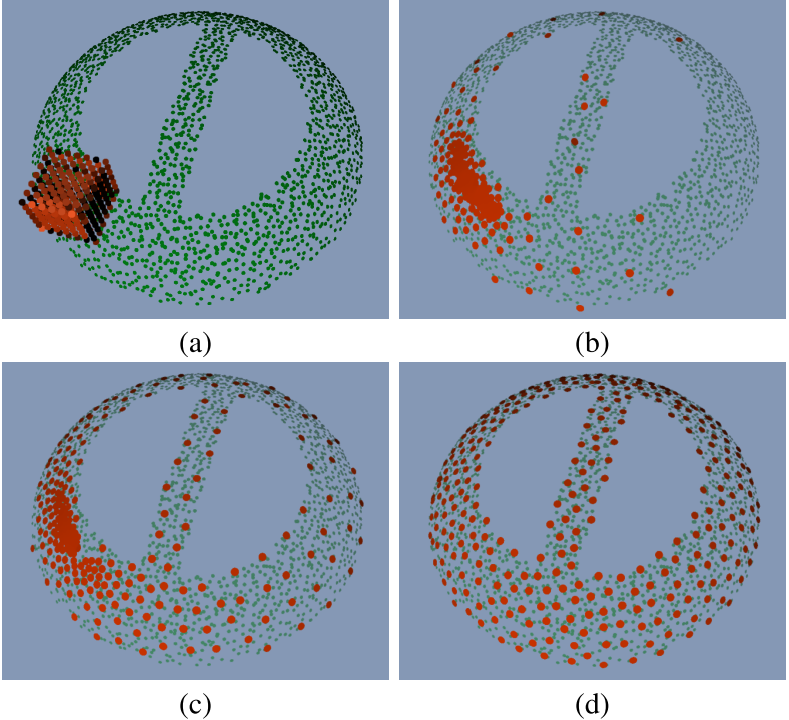
\includegraphics[width=2.5in]{images/L1median}
  \caption{Reconstruction by projection operation. (a). noisy point-set P(green) and an arbitrary point-set Q(red) that will be projected to P to approximate P. (b),(c) are two iterative projection results. (d) is the final projection.}
\end{figure}

Reconstruction by a projection operator, as shown in figure.., is to approximate the origin point-set(green) by iteratively projecting an arbitrary point-set(red) onto itself while removing the noises or outliers.
It has an important virtue: it defines a consistent geometry based on the data points, and provides constructive means to up-sample it.

A new projection operator is introduced via a certain fixed-point iteration where the approximated geometry consists of its stationary points,
and it is closely related to the $L_1$ median\cite{brown1983statistical,small1990survey} which is a statistical tool that applied globally to multivariate non-parametric point-samples in the presence of noise and outliers.
Briefly, it is a robust global center of an arbitrary set of points. Mathematically, given a data set $P=\{p_{j}\}_{j\in J}\subset \mathbb{R}^3$, the $L_1$ median is defined as the point $q$ obtained by minimizing the sum of Euclidean distances to the data points

\small{
\begin{equation}
 \label{eq:L1median}
 q=\arg\min_{x}\left\{ \sum_{j\in J}^{}\|p_{j}-x\| \right\}
\end{equation}
}

\paragraph{(1)}\cite{lipman2007parameterization} applies this tool locally to constitute a robust reconstruction mechanism called parameterization-free local projection operator(LOP). Starting with an arbitrary initial point-set $X^{(0)}=\{{x_{i}}^{(0)}\}_{i\in I}\subset \mathbb{R}^3$(typically $|X|\ll|P|$, $|\cdot|$ is the number of point-set), LOP computes the target point positions $X$ by performing a fixed-point iteration

\small{
\begin{equation}
 \label{eq:LOP1}
 X^{k+1}=\mathop{\argmin}_{X=\{x_{i}\}_{i\in I}}\{E_1(X^{k},P)+E_2(X^{k})\},\\
\end{equation}
}
\\
where,
\small{
\begin{equation}
 \label{eq:LOP2}
 \begin{split}
 & E_1(X^{k},P)=\sum_{i\in I}^{}\sum_{j\in J}^{}\|x_{i}-p_{j}\|\theta(\|x{_i^k}-p_{j}\|),\\
 & E_2(X^{k})=\sum_{i'\in I}^{}\lambda_{i'}\sum_{i\in I\setminus\{i'\}}^{} \eta(\|x_{i}-x{_{i'}^k}\|)\theta(\|x{_i^k}-x{_{i'}^k}\|).
 \end{split}
\end{equation}
}
\\
The term $E_1$ is in fact a localized version of () by using a fast-decaying weight function $\theta(r)=e^{-r^2/(h/4)^2}$ with the finite support radius $h$,
and thus it is just $E_1$ that drives the projected points $X$ to approximate the geometry of $P$.
The term $E_2$ keeps the distribution of the points $X$ fair by incorporating local repulsion forces.

Let $\xi{_{ij}^k}=x{_i^k}-p_{j}$ and $\delta{_{ii'}^k}=x{_i^k}-x{_{i'}^k}$, solving (), the projection for point $x{_i^{k+1}}$ is obtained as

\small{
\begin{equation}
 \label{eq:WLOP1}
 \begin{split}
 & x{_i^{k+1}}=\sum_{j\in J}^{}p_{j}\frac{\alpha{_{ij}^k}}{\sum_{j\in J}^{}\alpha{_{ij}^k}}+ \\
 &~~~~~~~~~~~\mu\sum_{{i'}\in I\setminus\{i\}}^{}\delta{_{ii'}^k}\frac{\beta{_{ii'}^k}}{\sum_{{i'}\in I\setminus\{i\}}^{}\beta{_{ii'}^k}},
 \end{split}
\end{equation}
}
\\
where, \small{
\begin{equation}
 \label{eq:WLOP2}
 \begin{split}
 & \alpha{_{ij}^k}=\frac{\theta(\|\xi{_{ij}^k}\|)}{\|\xi{_{ij}^k}\|}, \\
 & \beta{_{ii'}^k}=\frac{\theta(\|\delta{_{ii'}^k}\|)|\eta'(\|\delta{_{ii'}^k}\|)|}{\|\delta{_{ii'}^k}\|}.
 \end{split}
\end{equation}
}

Intuitively, LOP distributes the points by approximating their $L_1$ median to achieve robustness to outliers and data noises without any local orientation information nor a local manifold assumption.
However, also because of the use of the local density parameter $h$, it may not work well when the distribution of the input points is highly non-uniform and can fail to converge.

\paragraph{(2)}
Like\cite{lipman2007parameterization}, many surface reconstruction methods try to obtain the resulted mesh without estimation of normals due to the unreliability because of the noisy data.
In fact, oriented normals at the points play a critical role in surface reconstruction and the estimation of normals requires the sampling points to be uniformly distributed.
\cite{huang2009consolidation} proposes a new consolidation technique whose central task is normal estimation.

To take advantage of the success of LOP in denoising and outlier removal, and simultaneously address the non-uniform distribution problem, they incorporate locally adaptive density weights into LOP, resulting in WLOP, they define the weighted local densities for each point $p_{j}$ in P and $x_{i}$ in X during the $k$th iteration by $v_{j}=1+\sum_{j'\in J\setminus\{j\}}^{}\theta(\|p_{j}-p_{j'}\|)$ and $w{_i^k}=1+\sum_{i'\in I\setminus\{i\}}^{}\theta(\|\delta{_{ii'}^k}\|)$, the projection for point $x{_i^{k+1}}$ finally becomes

\small{
\begin{equation}
 \label{eq:WLOP1}
 \begin{split}
 & x{_i^{k+1}}=\sum_{j\in J}^{}p_{j}\frac{\alpha{_{ij}^k}/v_{j}}{\sum_{j\in J}^{}(\alpha{_{ij}^k}/v_{j})}+ \\
 &~~~~~~~~~~~\mu\sum_{{i'}\in I\setminus\{i\}}^{}\delta{_{ii'}^k}\frac{w{_{i'}^k}\beta{_{ii'}^k}}{\sum_{{i'}\in I\setminus\{i\}}^{}(w{_{i'}^k}\beta{_{ii'}^k})},
 \end{split}
\end{equation}
}
\\
The weighted local density $v$ in the first term relaxes the attraction of point clusters and repulsion force in dense areas is strengthened by the local density $w$ in the second term.

So far, we actually have obtained a reconstructed point set which will then be used to improve the reliability of normal initialization that will be used in a second normal estimation phase.
However, considering the high computational effort, it may not be a preferable choice using this consolidation technique as a preprocessing method for surface reconstruction even though some high quality surface can be reconstructed.


\paragraph{(3)}
In LOP/WLOP, the majority of the time is spent on the evaluation of the attractive forces from all points in $P$,
so \cite{preiner2014CPF} efficiently reduce the set $P$ of unordered input points to a much more compact mixture of Gaussians $\mathcal{M}=\{w_{s},\Theta_{s}\}$ that reflects the density distribution of the points.
That is, $\mathcal{M}$ defines a probability density function(pdf) as a weighted sum of $|\mathcal{M}|$ Gaussian components

\small{
\begin{equation}
 \label{eq:TV}
 f(\mathbf{x}|\mathcal{M})=\sum_{s}^{}w_{s}g(\mathbf{x}|\Theta_{s}),
\end{equation}
}
\\
where the $\Theta_{s}=(\mu_{s},\sum_{s}^{})$ are the Gaussian parameters, $w_{s}$ their corresponding convex weights, and $g$ denotes the $d$-variate Gaussian pdf with $g(\mathbf{x}|\mu,\sum)=|2\pi\sum_{}^{}|^{-\frac{1}{2}}e^{-\frac{1}{2}(\mathbf{x}-\mu)^{T}\sum_{}^{-1}(\mathbf{x}-\mu)}$.


a novel $continuous$ formulation of the WLOP operator based on a Gaussian mixture used for describing the input point density.


cannot address the missing data problem like LOP. This method is up to 7 times faster than an optimized GPU implementation of WLOP, and achieves interactive frame rates for moderately sized point clouds.

\subsubsection{Total variation(TV) based}
TV has been a popular tool for image processing tasks, such as denoising, reconstruction, and segmentation\cite{chambolle2010introduction}, the underlying model for TV methods also aims at exploiting the sparsity of the gradient of the image just like the idea of image smoothing\cite{xu2011image} mentioned above. The discrete variant yields the following convex objective function

\small{
\begin{equation}
 \label{eq:TV}
 TV(u)=\sum_{i,j}^{}\|D_{i,j}u\|_2
\end{equation}
}
\\
where $D_{i,j}$ is the discrete gradient operator at pixel $(i,j)$ and $u$ is a vector containing the gray-level pixel values. TV methods filter the image by minimizing $TV(u)$ which is in fact the $l_1$ norm of the vector $[\cdots~\|D_{i,j}u\|_2~\cdots]$.

Since TV is designed for images, it is not directly applicable to geometry processing problem. As we have stated, the key point is to find some form of second order information. Similar to the sparse gradient minimization, and based on the observation that the gradients of smooth surface normals are sparse, \cite{avron2010L1} formulates their piecewise smoothness reconstruction problem as a sparse minimization of orientation differences and position projections as following

\small{
\begin{equation}
 \label{eq:L1reconstruction}
 \begin{aligned}
 &N^{out} =\mathop{\argmin}_{N} \sum_{(p_{i},p_{j})\in E}^{} w_{i,j}\|n_{i}-n_{j}\|_2\\
 &s.t.~\forall i~\|n_{i}-{n_{i}}^{in}\|_2\le \gamma_{n} %~~~~~~~~
 \end{aligned}
\end{equation}
}
\small{
\begin{equation}
 \label{eq:L1reconstruction}
 X^{out} = \mathop{\argmin}_{X} \sum_{(p_{i},p_{j})\in E}^{} w_{i,j}|n_{i,j}\cdot (x_{i}-x_{j})|
\end{equation}
}

Convexity of these two problems allows for finding a global optimum and deriving efficient solvers. Figure..(d) shows a well reconstructed example with sharp features. Due to the global nature, this algorithm is extremely slow. And it may fail for the point set with severe noises and outliers.

\begin{figure}[ht]
  \centering
  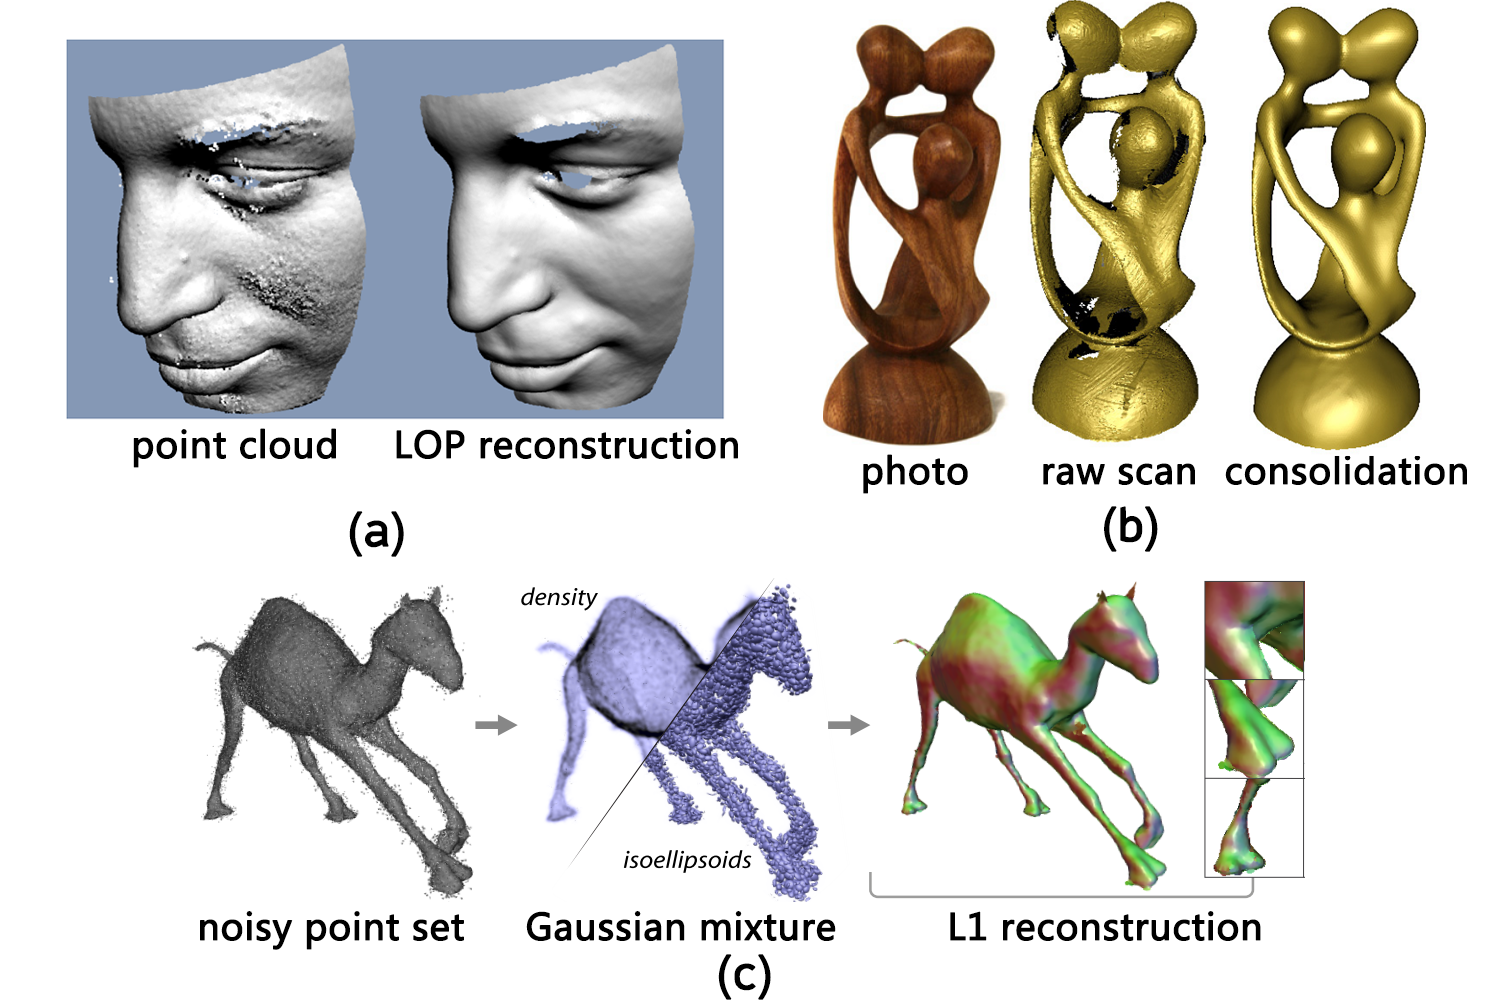
\includegraphics[width=3in]{images/reconstruction_L1}
  \caption{Sparse regularization: point cloud consolidation. (a): LOP\cite{lipman2007parameterization}. (b): WOLP\cite{huang2009consolidation}. (c): continuous WLOP\cite{preiner2014CPF}. (d): TV based\cite{avron2010L1}.}
\end{figure}


%\begin{equation}
% \label{eq:LOP}
% \begin{split}
% & Q=\arg\min_{x=\{x_{i}\}_{i\in I}}\{E_1(X,P,Q)+E_2(X,Q)\},\\
% & where \\
% & E_1(X,P,Q)=\sum_{i\in I}^{}\sum_{j\in J}^{}\|x_{i}-p_{j}\|\theta(\|q_{i}-p_{j}\|),\\
% & E_2(X,Q)=\sum_{i'\in I}^{}\lambda_{i'}\sum_{i\in I\setminus\{i'\}}^{} \eta(\|x_{i'}-q_{i}\|)\theta(\|q_{i'}-q_{i}\|).
% \end{split}
%\end{equation} 